\documentclass[11pt,a4paper]{article}
\usepackage{amsmath}
\usepackage{amssymb}
\usepackage{graphicx}
\usepackage{verbatim}
\begin{document}
\noindent
Martin Lundfall, Henri Bunting, Malte Siemers, Patrik Bey
\begin{centering}
  \section*{Exercise sheet 10 - Machine Intelligence I}
  \end{centering}
  
  \subsection*{10.1 - Directed Acylic Graphs and Graphical Models}
  
  \subsubsection*{(a)} Nodes represent the random variables, edges the correlative relationship between those nodes, and the edge direction symbolizes causation.
  \subsubsection*{(b)} Two nodes are conditionally independent if their combined probability, given a parent, is equal to the product of individual probabilities of the nodes given the parent.  This enables a decomposition of the graph.  Conditional Independence is shown in the graph structure as a lack of edges between nodes. 
  \newpage
  \subsubsection*{(c)} 
  Here is a step-by-step visualization of the algorithm.\\
  \begin{figure*}[h]
  	\begin{minipage}[t]{4 cm}
		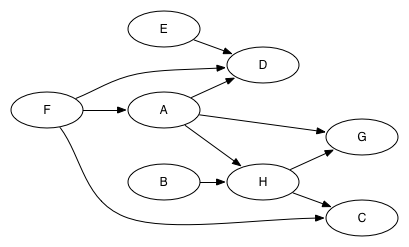
\includegraphics[width=\linewidth]{101c0}
		\caption{initial state}
  	\end{minipage}
  	\begin{minipage}[t]{4 cm}
		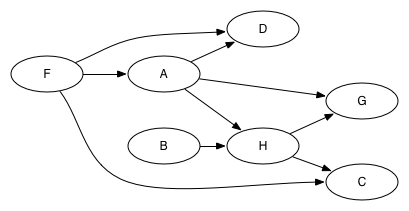
\includegraphics[width=\linewidth]{101c1}
		\caption{i = 1}
  	\end{minipage}
  	\begin{minipage}[t]{4 cm}
		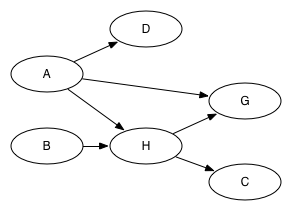
\includegraphics[width=\linewidth]{101c2}
		\caption{i = 2}
  	\end{minipage}
  	\begin{minipage}[t]{4 cm}
		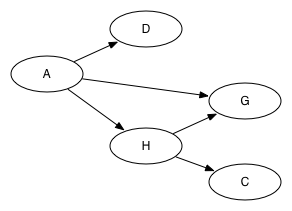
\includegraphics[width=\linewidth]{101c3}
		\caption{i = 3}
  	\end{minipage}
  	\begin{minipage}[t]{4 cm}
		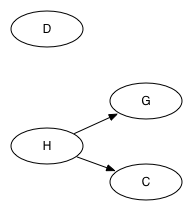
\includegraphics[width=\linewidth]{101c4}
		\caption{i = 4}
  	\end{minipage}
  	\begin{minipage}[t]{4 cm}
		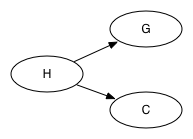
\includegraphics[width=\linewidth]{101c5}
		\caption{i = 5}
  	\end{minipage}
  	\begin{minipage}[t]{4 cm}
		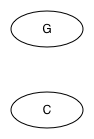
\includegraphics[width=\linewidth]{101c6}
		\caption{i = 6}
  	\end{minipage}
  	\begin{minipage}[t]{4 cm}
		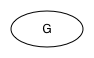
\includegraphics[width=\linewidth]{101c7}
		\caption{i = 7}
  	\end{minipage}
  \end{figure*}\\
  This results in the topological sorting: E,F,B,A,D,H,C,G
  \newpage
  \subsubsection*{(d)} The factorization of join distribution for the DAG is:\\
  $P(F) * P(E) * P(B) * P(A|F) * P(D|E,A,F) * P(H|B,A,F) * P(G|H,B,A,F) * P(C|H,B,A,F)$\\
  Given conditional independence, this can be reduced to:\\
  $P(F) * P(E) * P(B) * P(A|F) * P(D|E,A) * P(H|B,A) * P(G|H,A) * P(C|H,F)$
  \subsubsection*{(e)} The Markov Blanket of the node, A, is: $\{F,B,E,D,H\}$\\
  Where:\\
  $\{F\}$ is the parent node\\
  $\{D,H\}$ are children nodes\\
  $\{B,E\}$ are the children's parents nodes
  \subsubsection*{(f)} A naive Bayes Classifier assigns a class label to a node $x$ based on the class's probability and the probability of the node belonging to that class.\\
  \begin{equation}
  	\bar{y} = \underset{k}{\text{argmax}} P(C_{k})\prod_{i}P(x_{i}|C_{k})
  \end{equation}
  
\end{document}